\documentclass[a4paper, 12pt]{article}
\usepackage{titling}
\usepackage{array}
\usepackage{booktabs}
\usepackage{enumitem}
\usepackage{graphicx}
\usepackage{subfigure}
\usepackage{hyperref}
\usepackage{amssymb}
\usepackage{listings}
\usepackage{xcolor}
\usepackage[framed,autolinebreaks,useliterate]{mcode}
\setlength{\heavyrulewidth}{1.5pt}
\setlength{\abovetopsep}{4pt}
\setlength{\parindent}{0pt}
\graphicspath{{.}}

\usepackage[margin=1in]{geometry}

% Must be after geometry
\usepackage{fancyhdr}
\pagestyle{fancy}
\fancyhf{}
\rhead{ECTA Homework 02}
\cfoot{\thepage}

\setlength{\droptitle}{-5em}

\title{Evolutionary Computation Theory and Application  \\
				- Assignment 2: Traveling Salesman Problem -}
\author{Debaraj Barua (9030412), Md Zahiduzzaman (9030432)}

\date{}

\begin{document}

\maketitle

\section{General Remarks }

Please Follow those remarks. Deviating will lead to a reduced score

\begin{itemize}
	\item Lable your axis 
	\item Include a descriptive, not covering legend in your plots
	\item Caption you images with a clear description
	\item Remember to name the file correctly
	\item Make sure that both team members submit the same file, with the same name
	\item Please make sure that all figures and lines are clearly readable
\end{itemize}

\section{Solution}
\begin{table} [h!]
	  \centering
\begin{tabular}{|l|l|}
\hline
\textbf{Parameter} & \textbf{Value}   \\
\hline
Population size & 50 \\
\hline
Crossover Rates &  1\%, 10\%, 99\%, 100\% \\
\hline
Mutation Rates & 1\%, 10\%, 99\%, 100\% \\
\hline
Repetitions & 30 \\
\hline
Generations & 1000 \\
\hline
Average best fitness		 & 108.1341 \\
\hline
Minimum best fitness		 & 69.8973 \\
\hline
\end{tabular}
\caption{99\% mutation rate used for various crossover rate and 99\% crossover rate used for various mutation rate. For 30 repetition, both crossover and mutation rate was set to 99\% }
\label{table:defparams}
\end{table}
\subsection{Details of Approach}
\begin{enumerate}
	%-------------------------%
	% Put your code here:
	
	\item \textbf{Tournament Selection}
	\lstinputlisting[firstline=30, lastline=45]{../src/my_selection.m}
	\textcolor{blue}{
	\begin{itemize}
		\item We select two groups of random individuals.
		\item We select the best performing individual from each group and choose these as the two parents.
	\end{itemize}
	}
	
	\item \textbf{Crossover}
	\lstinputlisting[firstline=29, lastline=58]{../src/my_crossover.m}
	\textcolor{blue}{
	\begin{itemize}
		\item We iterate over each individual in the population and check if we should use crossover using the crossover probability.
		\item If False, we use the first parent as the child.
		\item If True, we select one random point in the gene and split it into two parts.
		\item We then create a new individual by selecting the first part from the first parent and the second part from the second parent.
	\end{itemize}
	}
	
	
	\item \textbf{Mutation}
	\lstinputlisting[firstline=24, lastline=48]{../src/my_mutation.m}
	\textcolor{blue}{
	\begin{itemize}
		\item We iterate over each individual in the population and check if we should mutate it using the mutation probability.
		\item If True, we select two random points in the gene and split it into three parts.
		\item We then create a new individual by reorganizing these three parts, as shown above.
	\end{itemize}	
	}
	
	\item \textbf{Elitism}
	\lstinputlisting[firstline=25, lastline=28]{../src/my_elitism.m}	
	\textcolor{blue}{
	\begin{itemize}
		\item From each generation, we save some best performing individuals, and forward them to the next generation. 
		\item This ensures that we do not loose all the best individuals to mutation and/or crossover. 
	\end{itemize}
	}
	
	%-------------------------%
	\end{enumerate}
\section{Results}

\begin{figure}[ht!]
  \centering
  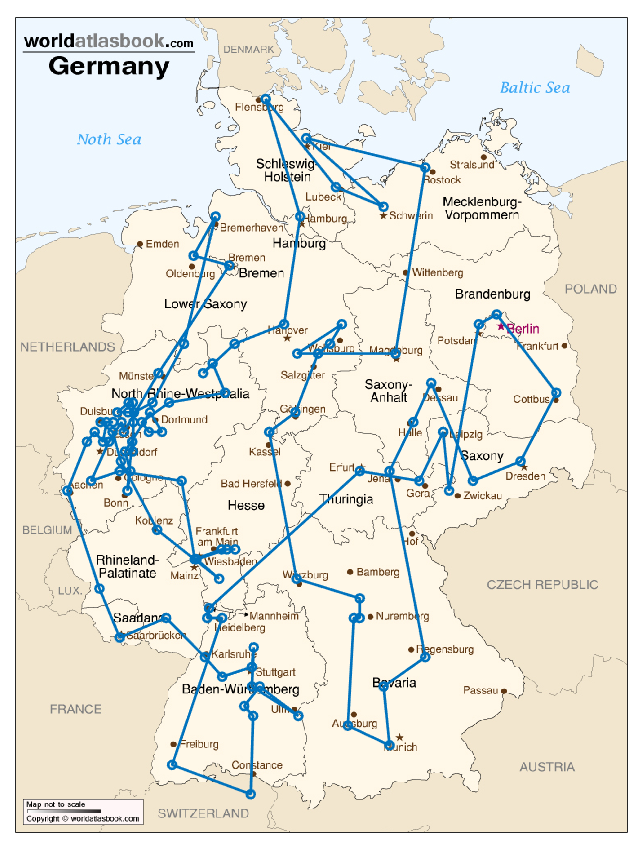
\includegraphics[width=1.0\textwidth]{images/resultmap-mine-crop}
    \caption{Map using 100\% crossover and 100\% mutation \label{fig:map}}
\end{figure}

\subsection{Different mutation rates}

\begin{figure}[ht!]
	\centering
	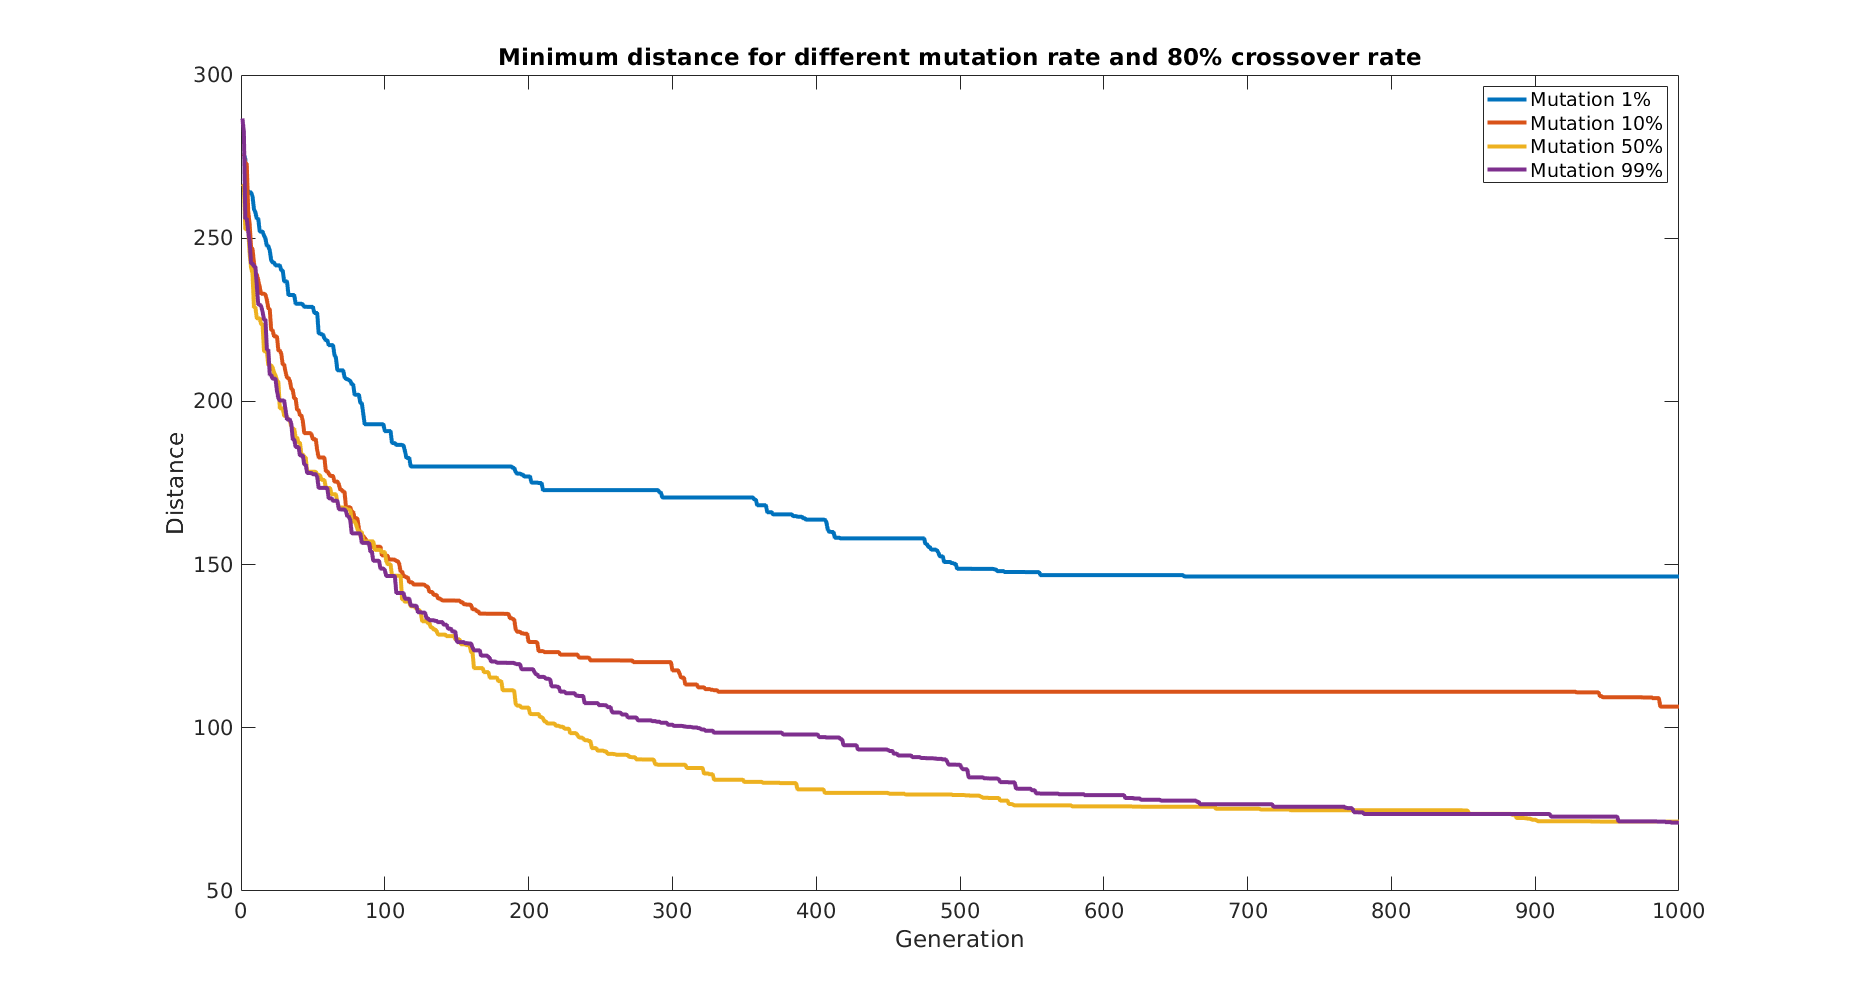
\includegraphics[width=1.1\textwidth]{images/mutfig-mine}
	\caption{Different mutation rate for 100\% crossover \label{fig:mutfig}}
\end{figure}

Describe and explain the different mutation rates and how they influence the learning behavior. Please remember to also focus on why, not only on what.
Also elaborate on the mutation rate you have chosen as best mutation rate.
\\ \\
\textcolor{blue}{
	\begin{itemize}
		\item From the graph above we see that the fitness improves as we increase the mutation rate.
		\item The complexity of problem with brute force is of the order of $O(n!)$. That is, we have a huge search space and thus to solve within a reasonable execution time, we need higher randomization or change. 
		\item Thus, we can conclude that using a higher mutation rate will avoid getting stuck in local minima and enable us to converge to a solution faster.
		\item Thus we select a mutation rate of $100\%$ as our best estimate of the mutation parameter. 
	\end{itemize}
	}

\subsection{Different crossover rates}


\begin{figure}[ht!]
  \centering
  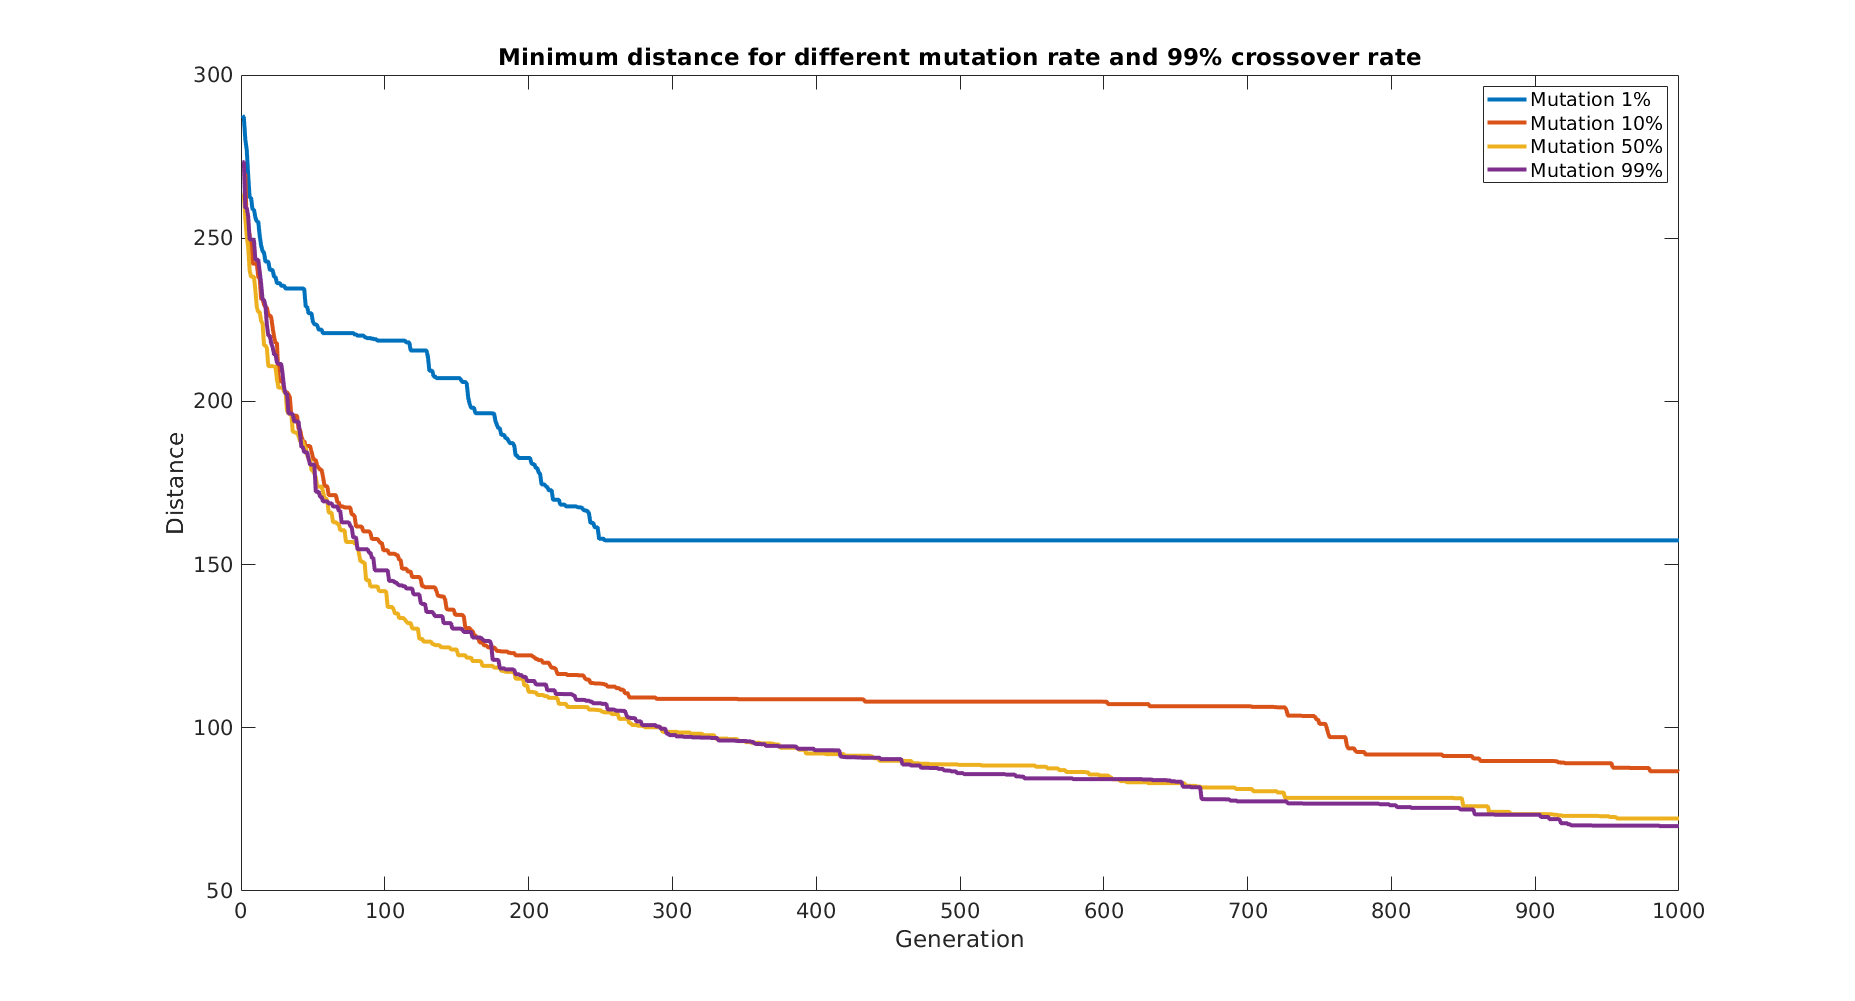
\includegraphics[width=1.0\textwidth]{images/crossfig-mine}
    \caption{Different crossover rate for 100\% mutation \label{fig:crossfig}}
\end{figure}

Describe and explain the different crossover rates and how they influence the learning behavior. Please remember to also focus on why, not only on what.
Also elaborate on the crossover rate you have chosen as best mutation rate.
\\ \\
\textcolor{blue}{
	\begin{itemize}
		\item As elaborated for the mutation rate, we observe that on increasing the crossover rate, we get better fitness values.
		\item Following a similar logic, we choose $100\%$ crossover rate as our best estimate.
		\item However, on comparing with the previous graph in Figure 2, we can observe that using a higher crossover rate results in converging to a better solution faster. 
		\item In Figure 3, we can also observe that for lower values of crossover, the fitness value does not saturate completely by 1000 generations.
		\item This can be reasoned as below:
			\begin{itemize}
				\item Crossover is preceded by the selection of parents.
				\item During this step, two groups of parents are selected and the best performing individuals from these groups are used as parents.
				\item Thus, it stands to reason that when our crossover rate is high, we are using better performing parents to potentially create better performing child.
				\item When our crossover is low, we forgo the possibility of using the fitness of previous generation, and must always rely on mutation. Thus leading to slower convergence.				
			\end{itemize}
	\end{itemize}
}



\end{document}
